\documentclass{article}
\usepackage{ctex}
\usepackage{graphicx}
\usepackage{amsmath,amsthm,amssymb}
\usepackage{newtxtext}
\usepackage[bookmarks=true, colorlinks, citecolor=blue, linkcolor=black]{hyperref}
\usepackage{geometry}
\usepackage{lipsum} % 该宏包是通过 \lipsum 命令生成一段本文,正式使用时不需要引用该宏包
\usepackage[dvipsnames,svgnames]{xcolor}
\usepackage[strict]{changepage} % 提供一个 adjustwidth 环境
\usepackage{framed} % 实现方框效果

\usepackage{tcolorbox}

% 中文定理环境
% \indent 为了段前空两格

\newtheorem{theorem}{\indent 定理}[section]
\newtheorem{lemma}[theorem]{\indent 引理}
\newtheorem{proposition}[theorem]{\indent 命题}
\newtheorem{corollary}[theorem]{\indent 推论}
\newtheorem{definition}{\indent 定义}[section]
\newtheorem{example}{\indent 例}[section]
\newtheorem{remark}{\indent 注}[section]
\newenvironment{solution}{\begin{proof}[\indent\bf 解]}{\end{proof}}
\renewcommand{\proofname}{\indent\bf 证明}

% % English theorem environment
% \newtheorem{theorem}{Theorem}[section]
% \newtheorem{lemma}[theorem]{Lemma}
% \newtheorem{proposition}[theorem]{Proposition}
% \newtheorem{corollary}[theorem]{Corollary}
% \newtheorem{definition}{Definition}[section]
% \newtheorem{remark}{Remark}[section]
% \newtheorem{example}{Example}[section]
% \newenvironment{solution}{\begin{proof}[Solution]}{\end{proof}}

\geometry{a4paper,centering,scale=0.8}
% environment derived from framed.sty: see leftbar environment definition
\definecolor{formalshade}{rgb}{0.95,0.95,1} % 文本框颜色
% ------------------******-------------------
% 注意行末需要把空格注释掉,不然画出来的方框会有空白竖线
\newenvironment{quoteblock}{%
\def\FrameCommand{%
\hspace{1pt}%
{\color{DarkBlue}\vrule width 2pt}%
{\color{formalshade}\vrule width 4pt}%
\colorbox{formalshade}%
}%
\MakeFramed{\advance\hsize-\width\FrameRestore}%
\noindent\hspace{-4.55pt}% disable indenting first paragraph
\begin{adjustwidth}{}{7pt}%
\vspace{2pt}\vspace{2pt}%
}
{%
\vspace{2pt}\end{adjustwidth}\endMakeFramed%
}
% ------------------******-------------------
\definecolor{greenshade}{rgb}{0.90,0.99,0.91} % 绿色文本框,竖线颜色设为 Green
\definecolor{redshade}{rgb}{1.00,0.90,0.90}% 红色文本框,竖线颜色设为 LightCoral
\definecolor{brownshade}{rgb}{0.99,0.97,0.93} % 莫兰迪棕色,竖线颜色设为 BurlyWood

\newenvironment{solblock}{%
\def\FrameCommand{%
\hspace{1pt}%
{\color{BurlyWood}\vrule width 2pt}%
{\color{brownshade}\vrule width 4pt}%
\colorbox{brownshade}%
}%
\MakeFramed{\advance\hsize-\width\FrameRestore}%
\noindent\hspace{-4.55pt}% disable indenting first paragraph
\begin{adjustwidth}{}{7pt}%
\vspace{2pt}\vspace{2pt}%
}
{%
\vspace{2pt}\end{adjustwidth}\endMakeFramed%
}

\newenvironment{quesblock}{%
\def\FrameCommand{%
\hspace{1pt}%
{\color{Green}\vrule width 2pt}%
{\color{greenshade}\vrule width 4pt}%
\colorbox{greenshade}%
}%
\MakeFramed{\advance\hsize-\width\FrameRestore}%
\noindent\hspace{-4.55pt}% disable indenting first paragraph
\begin{adjustwidth}{}{7pt}%
\vspace{2pt}\vspace{2pt}%
}
{%
\vspace{2pt}\end{adjustwidth}\endMakeFramed%
}



% ------------------define markerblock-------------------
\tcbuselibrary{most} 
\newtcolorbox{markerblock}[1][]{enhanced,
  before skip=2mm,after skip=3mm,
  boxrule=0.4pt,left=5mm,right=2mm,top=1mm,bottom=1mm,
  colback=yellow!20,
  colframe=yellow!40!black,
  sharp corners,rounded corners=southeast,arc is angular,arc=3mm,
  underlay={%
    \path[fill=tcbcolback!80!black] ([yshift=3mm]interior.south east)--++(-0.4,-0.1)--++(0.1,-0.2);
    \path[draw=tcbcolframe,shorten <=-0.05mm,shorten >=-0.05mm] ([yshift=3mm]interior.south east)--++(-0.4,-0.1)--++(0.1,-0.2);
    \path[fill=yellow!80!black,draw=none] (interior.south west) rectangle node[white]{\Huge\bfseries !} ([xshift=4mm]interior.north west);
    },
  drop fuzzy shadow,#1}

% ---------------define tips--------------

\definecolor{tipscolor}{rgb}{0.77,0.72,0.65} % 莫兰迪棕色
\newtcolorbox{tipsblock}[2][]
{enhanced,breakable,
left=12pt,right=12pt,% 左右边距
% fonttitle=\bfseries, % 可以设置标题是否粗体
coltitle=white, % 标题字体颜色
colbacktitle=tipscolor, % 标题背景颜色
attach boxed title to top left={yshifttext=-1mm},
boxed title style={skin=enhancedfirst jigsaw,arc=1mm,bottom=0mm,boxrule=0mm},
boxrule=1pt, % 边框线宽
colback=OldLace, % 文本框背景颜色
colframe=tipscolor, % 框线颜色
sharp corners=northwest,
% drop fuzzy shadow, % 可以选择是否设置阴影效果
title=\vspace{3mm}\textbf{#2},
arc=1mm,
#1}
% ------------------******-------------------
\newenvironment{thmblock}[1][\textbf{Theorem}]{\begin{tcolorbox}[title=\textbf{#1}, colback=red!5,colframe=red!75!black]}{\end{tcolorbox}}

\newenvironment{defblock}[1][\textbf{Definition}]{\begin{tcolorbox}[colback = Emerald!10, colframe = cyan!40!black, title = \textbf{#1}]}{\end{tcolorbox}}

\newenvironment{lemmablock}[1][\textbf{Lemma}]{\begin{tcolorbox}[title=\textbf{#1},colback=SeaGreen!10!CornflowerBlue!10,colframe=RoyalPurple!55!Aquamarine!100!]}{\end{tcolorbox}}

\newenvironment{propblock}[1][\textbf{Proposition}]{\begin{tcolorbox}
[title = \textbf{#1}, colback=Salmon!20, colframe=Salmon!90!Black]}{\end{tcolorbox}}

\newenvironment{colblock}[1][\textbf{Collary}]{\begin{tcolorbox}[colback=JungleGreen!10!Cerulean!15,colframe=CornflowerBlue!60!Black,title = \textbf{#1}]}{\end{tcolorbox}}
% ----------------*******---------------

\usepackage{fancyhdr}
\usepackage{lastpage}
\fancypagestyle{plain}{
\fancyhf{}
\lhead{2023}
\chead{\centering{Notes of Machine Learning}}
\rhead{\thepage\ of \pageref{LastPage}}
\lfoot{}
\cfoot{}
\rfoot{}}
\pagestyle{plain}



% --------------Basic Information-----------

\title{\textbf{{Machine Learning}}}
\author{Chenxu Wang}
\date{\today}


% ------------------******-------------------
\begin{document}
\maketitle

\section{Machine Learning}

\begin{colblock}[Definition of Machine Learning]
    At the start of this class, one define Machine Learning is automatically find the function which could address our question.
\end{colblock}

So how do you tell the machine what function you're looking for?

\subsection{Supervised Learning}

Need to be supplied to machine Labeled data. Calculate the Loss of the corresponding Function to determine whether it is good or bad.

\subsection{Reinforcement Learning}


Let the machine find its own strategy, and only Reward the machine to guide the learning.

\section{Regression - Case Study}


Take Pokemon's Combat Power. Find a Function that predicts the evolutionary CP value. Namely:

$$
f(x)=CP_{after}\quad (x \quad \text{is Pokemon's all info})
$$

\begin{enumerate}
    \item Model

    Let's assume that this function is $y = b + w \cdot x_{cp}$ Where $b$, $w$ can take any value.

    \begin{colblock}[Definition of Linear Model]
    $x_i$ : an attribute(or feature) of input x.\\
    $w_i$ : weight.\\
    $b$ : bias.
    $$
    y = b + \sum w_i x_i
    $$
    \end{colblock}

    \item Goodness of Function

    There exist many real data. Denoted as: $(x^1,\hat{y}^1),\cdots,(x^{10},\hat{y}^{10})$ .

    To evaluate the Function, we define a loss function $L$. Input: a \textbf{function}, Output: how \textbf{bad} it is.

    $$
    L(f) = L(w,b)= \sum_{n=1}^{10}\left( b+\left(w \cdot x_{c p}^{n}\right)\right)^{2}
    $$

    Now we should use the loss function to pick the best Function in model function set out

    We denote the function as:

    $$
    f^*=arg \min_f L(f)
    $$

     $$
    w^*,b^*=arg \min_{w,b} L(w,b)
    $$

    And how to solve the target function out?

    \item Gradient Descent

    A new method the solve this equation: \textbf{Gradient Descent}.

    \begin{propblock}[How To Use Gradient Descent]
        \begin{itemize}
            \item In $\mathbb{R}$
            
            \begin{itemize}
                \item Randomly pick an initial value $w^0$
                
                \item Compute $\left.\frac{d L}{d w}\right|_{w=w^{0}}$

                If value is negative we should increase $w$. Otherwise decrease $w$.
    
                \item Parameter update: $w^0-\eta \left.\frac{d L}{d w}\right|_{w=w^{0}}\to w^1$ the $\eta$ is called \textit{learning rate}.
    
                \item Compute $\left.\frac{d L}{d w}\right|_{w=w^{1}}$
    
                \item Many iteration...
    
                \item we get the Local Minimum (Local Optimal). But in Linear Regression, There is no Local Optimal in the function.
            \end{itemize}
            
            \item In $\mathbb{R}^n$

            \begin{itemize}
                \item Randomly pick an initial value $w^0,b^0$
                
                \item Compute $\left.\frac{\partial L}{\partial w}\right|_{w=w^{0}, b=b^{0}},\left.\frac{\partial L}{\partial b}\right|_{w=w^{0}, b=b^{0}}$
    
                \item Parameter update: $w^0-\eta\left.\frac{\partial L}{\partial w}\right|_{w=w^{0}, b=b^{0}}\to w^1$ ,$b^0-\eta\left.\frac{\partial L}{\partial b}\right|_{w=w^{0}, b=b^{0}}\to b^1$ 
    
                \item Many iteration...
    
                \item Equally, in Linear Regression the loss function $L$ is convex. Also called no Local Optimal.
            \end{itemize}
        \end{itemize} 
    \end{propblock}

    \begin{tipsblock}{Gradient}
    
        $$
        \nabla L = \begin{bmatrix} \frac{\partial L}{\partial w} \\ \frac{\partial L}{\partial b}\end{bmatrix}
        $$
        
    \end{tipsblock}

    By calculating, we get $b=-188.4,w=2.7$ and errors in training data is $\sum e^n = 31.9$.
    
    Actually, we don't care errors in training data.What we really care about is the error on new data (testing data).

    So, we get another 10 Pokemon as testing data. The errors is $\sum e^n = 35.0 >$ training data error.

    \item Model Selection

    How can we do better?
    
    We select a new model: 
    $y=b+w_1\cdot x_{cp}+w_2\cdot(x_{cp})^2$
    And so on... 

    But when the selected function is complex, the testing error will increase instead. This phenomenon is called \textbf{Overfitting}.

    In fact, when we get enough data, we find that the Pokemon species is the main cause of CP values.So back to step 1, redesign the model.

    $$
    \delta(x_s=\text{A})=\begin{cases}
     1 & \text{ if } x_s=\text{A}\\
     0 & \text{Otherwise}
    \end{cases}
    $$

    $$
    \begin{aligned} y= & b_{1} \cdot \delta\left(x_{s}=\text { Pidgey }\right) \\ & +w_{1} \cdot \delta\left(x_{s}=\text { Pidgey }\right) x_{c p} \\ & +b_{2} \cdot \delta\left(x_{s}=\text { Weedle }\right) \\ & +w_{2} \cdot \delta\left(x_{s}=\text { Weedle }\right) x_{c p} \\ & +b_{3} \cdot \delta\left(x_{s}=\text { Caterpie }\right) \\ & +w_{3} \cdot \delta\left(x_{s}=\text { Caterpie }\right) x_{c p} \\ & +b_{4} \cdot \delta\left(x_{s}=\text { Eevee }\right) \\ & +w_{4} \cdot \delta\left(x_{s}=\text { Eevee }\right) x_{c p}\end{aligned}
    $$

    We will also consider whether other information about Pokemon may also influence the prediction of CP values. So we add a lot of other variables to form new functions:

    $$
    y^{\prime}=b_{1}+w_{1} \cdot x_{c p}+w_{2} \cdot\left(x_{c p}\right)^{2}
    $$

    $$
    y=y^{\prime}+w_{3} \cdot x_{h p}+w_{4} \cdot\left(x_{h p}\right)^{2}+w_{5} \cdot x_{h}+w_{6} \cdot\left(x_{h}\right)^{2}+w_{7} \cdot x_{w}+w_{8} \cdot\left(x_{w}\right)^{2}
    $$

    But this model is Overfitting. We back to step 2, to \textit{Regularization}. We define the loss Function is:

    $$
    L=\sum_{n}\left(\hat{y}^{n}-\left(b+\sum w_{i} x_{i}\right)\right)^{2}+\lambda \sum\left(w_{i}\right)^{2}
    $$

    The reason we added $\lambda$ is to smooth out its function so that it is not too sensitive to changes in data.At the same time, we don't need to put the bias in it. The value of $\lambda$ need us to test it out by hand.
\end{enumerate}

\section{Basic Concept}

Where is the error come from? When we really know where the error comes from, we can take targeted solutions.

Exist a unique perfect function $\hat f$. The only things we could do is let the $f^*$ which come from training data be closer to $\hat f$. And the distance from $\hat f$ to $f^*$ consist of Bias and Variance.

\subsection{Bias and Variance of Estimator}

The composition of the difference between the two functions is shown in the figure below.

\begin{figure}[htbp]
  \centering
  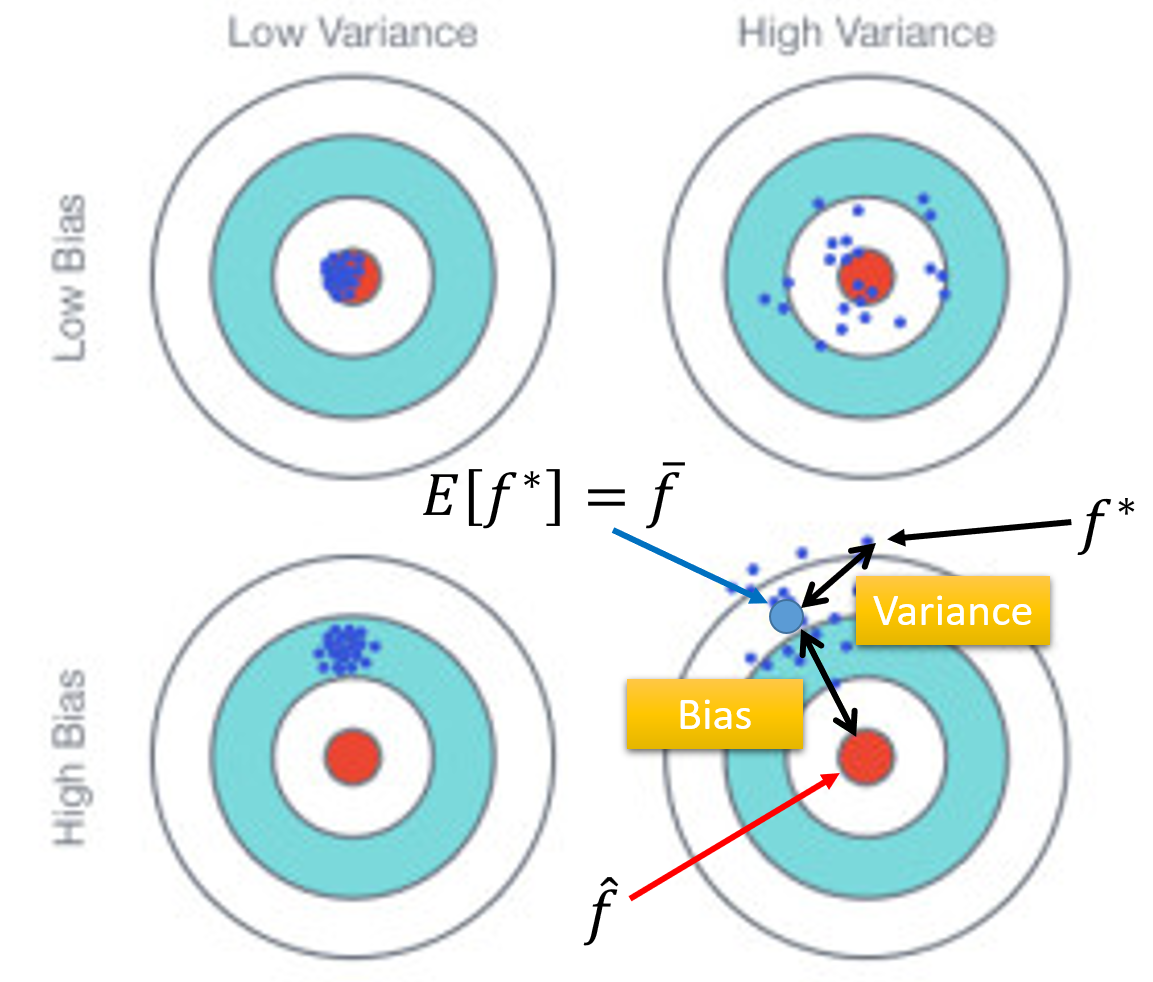
\includegraphics[scale=0.6]{pic/difference.png}
  \label{fig:my_label}
\end{figure}

In a word sum up how to judge which of the two causes of the error. Before we judge, we need to know that in the same model, different initial data will produce different functions.

When we have enough initial data sets, averaging the functions of each set yields an average function close to the perfect function.When the difference between the average function and the perfect function is larger, the problem appears on bias.

Your Function sets like the blue circle. The lager set you have the less loss in bias. Because the blue circle include the target function.

\newpage

\begin{figure}[htbp]
  \centering
  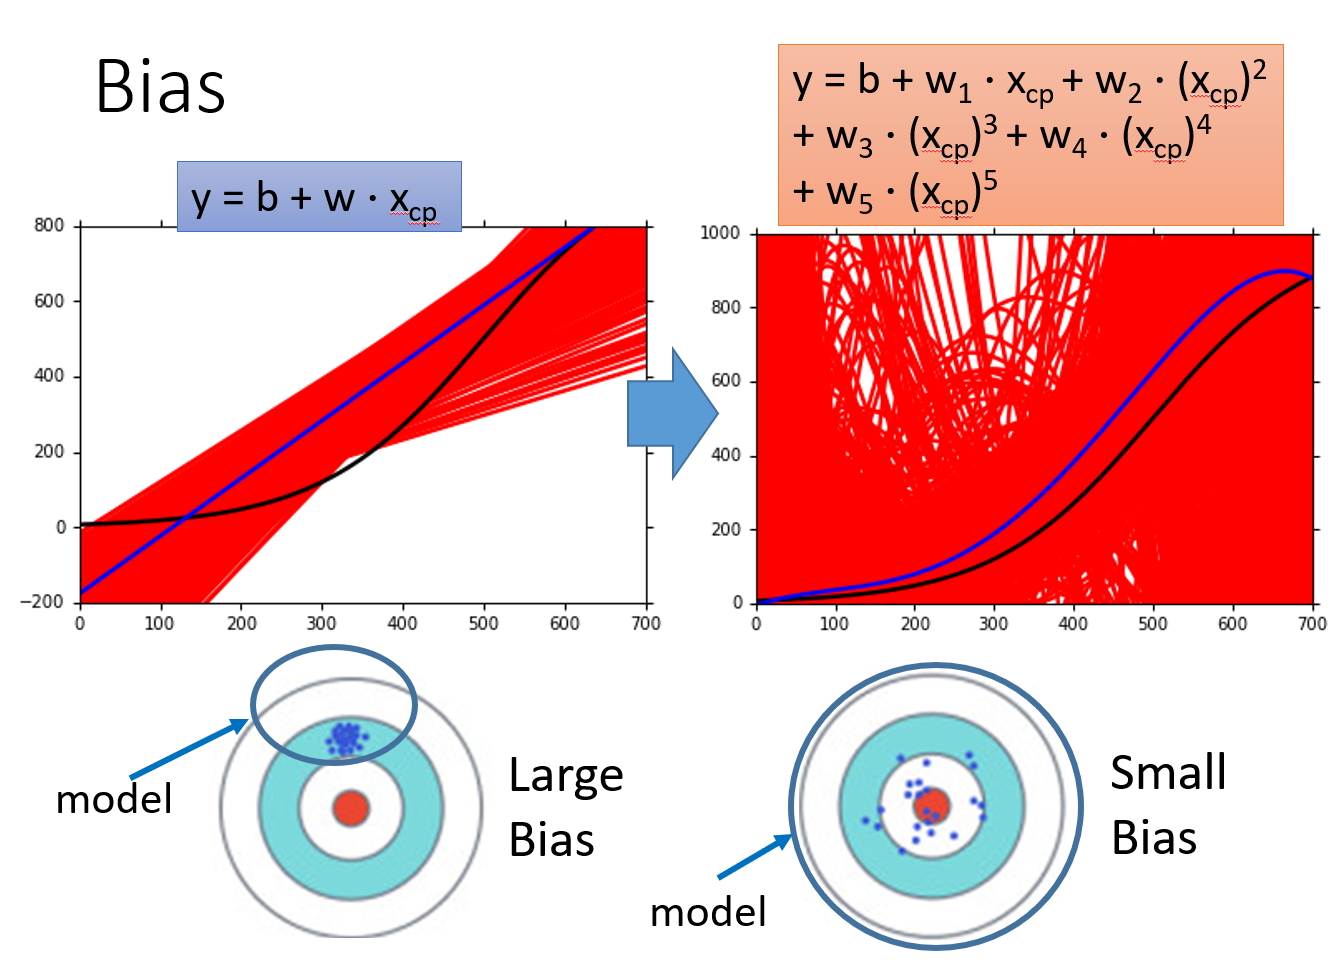
\includegraphics[scale=0.5]{pic/Bias.png}
  \label{fig:my_label}
\end{figure}

And next is variance. It seems that the average bias of a quintic function is small enough. But in the test data there will be a larger error, that is, the picture of the data point is not concentrated enough.

There are two ways to solve this problem, one is to simplify the model, the other is to smooth the model.

\begin{figure}[htbp]
  \centering
  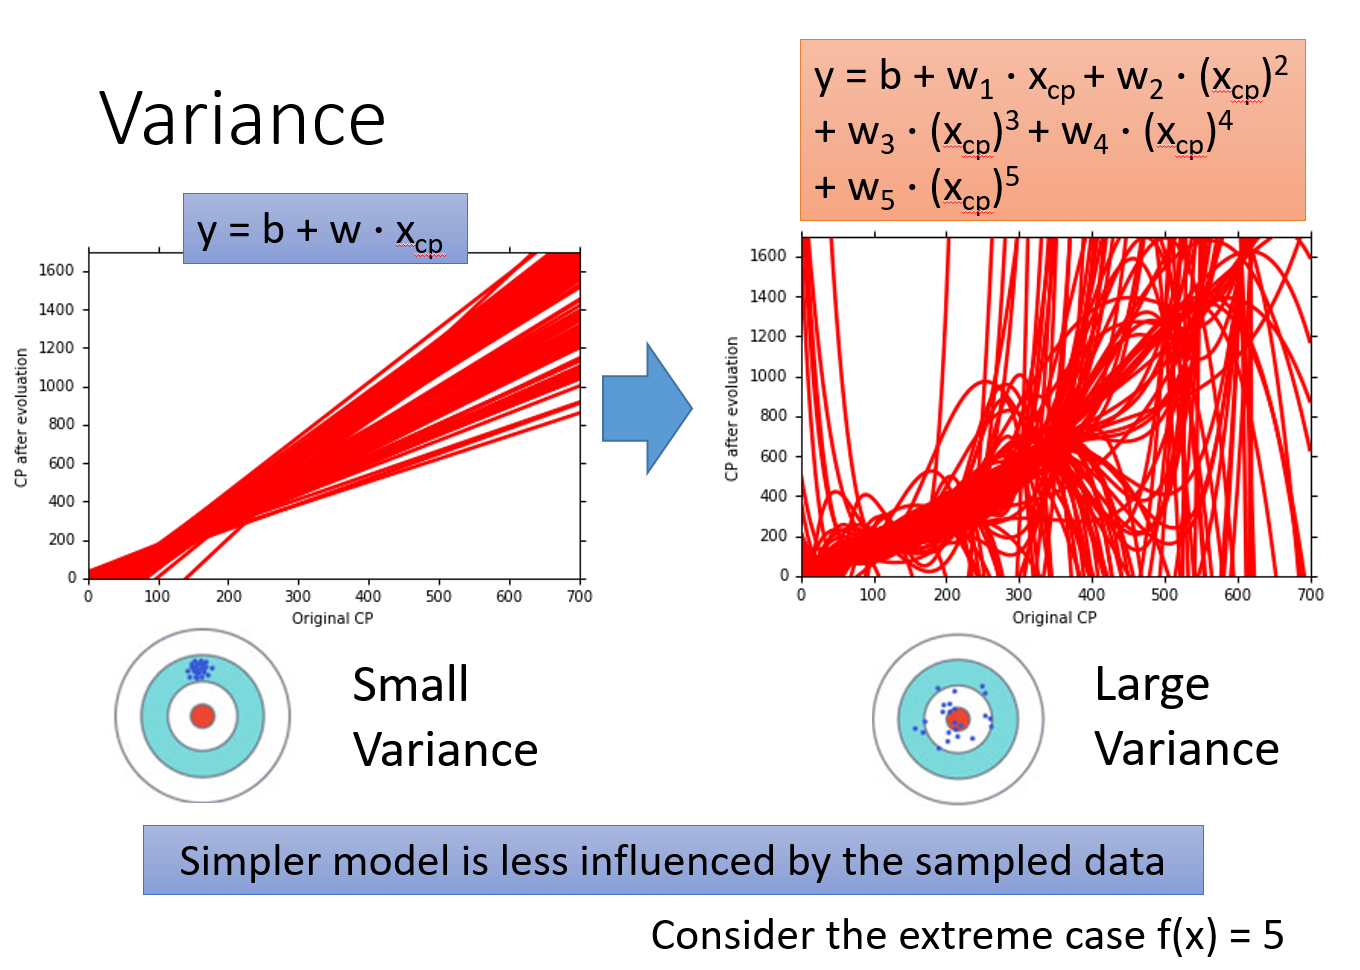
\includegraphics[scale=0.5]{pic/Variance.png}
  \label{fig:my_label}
\end{figure}

\section{Gradient Descent}

In step 3, we have to solve the following optimization problem:
$$
\theta ^* = arg \min_\theta L(\theta) 
$$
$L$: loss function \ $\theta$: parameters

Suppose that $\theta$ in $\mathbb{R} ^ n$. Randomly start at $\theta^0$. And do iterate:$\theta^{n+1} = \theta^n - \eta \nabla L(\theta^n)$ .

\subsection{Tuning Learning Rates}

There is a popular \& simple idea: Reduce the learning rate by some factor every few epochs. At the beginning, we are far from the destination, so we use larger learning rate. After several epochs, we are close to the destination, so we reduce the learning rate. There is an example:
$$
\eta ^ t = \frac{\eta}{\sqrt{t + 1}}
$$
Learning rate cannot be one-size-fits-all. Giving different parameters different learning rates.

\subsubsection{Adagrad Method}

\begin{colblock}[Definition of Adagrad Method]
    Divide the learning rate of each parameter by the \textbf{root mean square} of its previous derivatives.
\end{colblock}

\begin{propblock}[How To Use Adagrad]
    Let $k^t$ is the t-th iteration's \textit{learning rates}, $\sigma^t$ is \textbf{root mean square} of the previous derivatives of parameter. Here is the learning rate above:
    
    $$
    w^{t+1} = w^t - k^tg^t= w^t - \frac{\eta^t}{\sigma^t}g^t\quad (\eta^t = \frac{\eta}{\sqrt{t+1}}\quad g^{t}=\frac{\partial L\left(w^{t}\right)}{\partial w})
    $$

    $$
    \sigma^t = \sqrt{\frac{1}{n+1}\sum_{i=0}^t(g^i)^2}\quad k^t = \frac{\eta}{\sqrt{\sum_{t=0}^{t}(g^i)^2}}
    $$
    
\end{propblock}

It can be mathematically proven that the best step size is $\frac{\partial L(x^t)/\partial x}{\partial^2 L(x^t)/\partial x^2}$ . In fact, the reciprocal of root mean square actually replaces the second partial derivative.

\subsection{Make Descent Faster}

There is another method of descent: \textbf{Stochastic Gradient Descent}. This is the opposite of the previous gradient descent. This method pick only one example in one time. Make loss function for only one example:
$$
L^n=\left(\hat{y}^n-\left(b+\sum w_ix_i^n\right)\right)^2
$$
$$
\theta^i=\theta^{i-1}-\eta\nabla L^n{\left(\theta^{i-1}\right)}
$$

\subsection{Make Data More Suitable}

Let's assume there's only two dimensions. When the range of data in one dimension is small and the range of data in the other dimension is large. In the process of gradient descent iteration, the optimization of function can not directly point to the optimal function. Therefore, we need \textbf{Feature Scaling}. 

\begin{figure}[htbp]
  \centering
  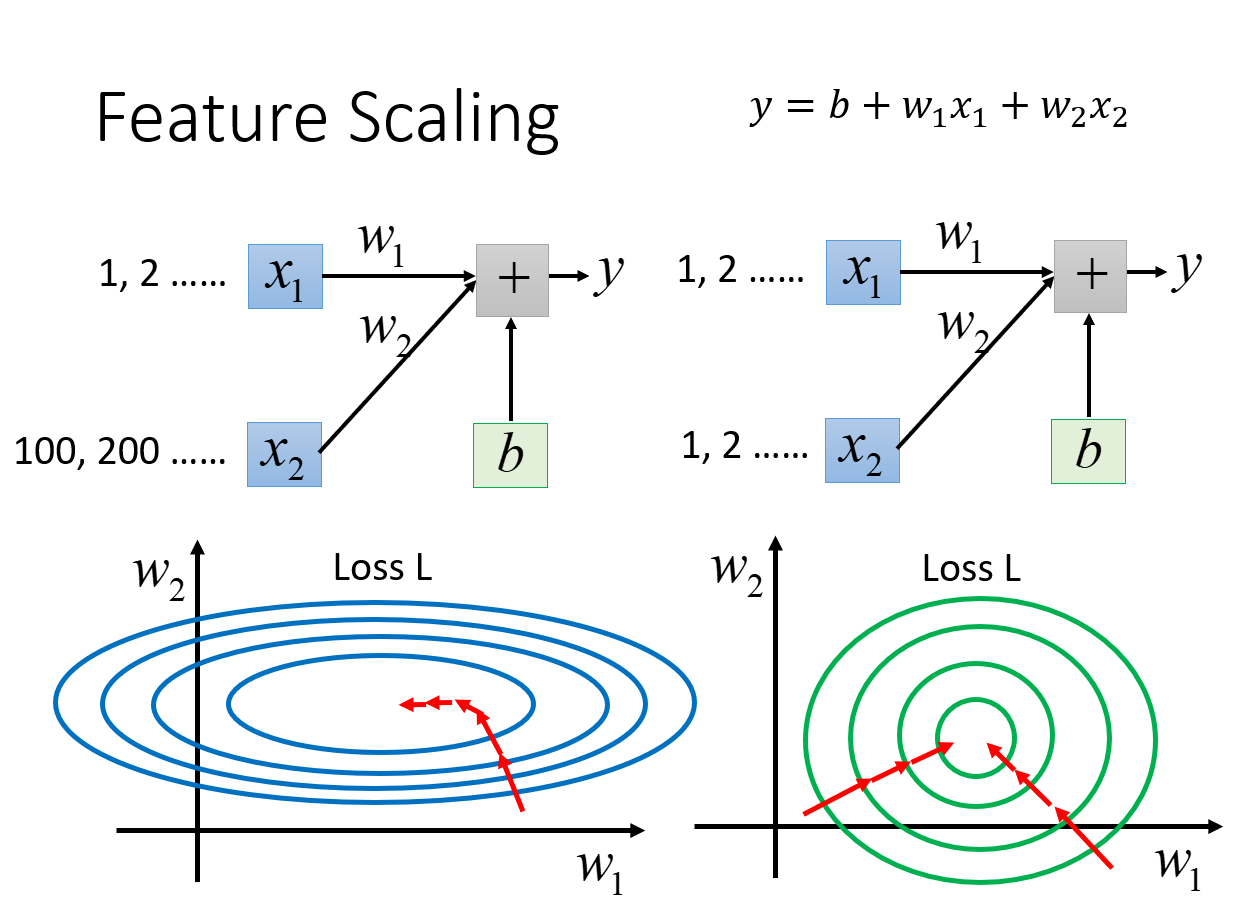
\includegraphics[scale=0.5]{pic/Feature Scaling.png}
  \label{fig:my_label}
\end{figure}

\begin{colblock}[Definition of Feature Scaling]
    Make different features have the same scaling.
\end{colblock}

\begin{propblock}[How To Do Feature Scaling]
    For each dimension $i$: mean: $m_i$, standard deviation: $\sigma_i$.
    
    For each point, new $x^i$ equal $\frac{x^i-x_i}{\sigma_i}$.
\end{propblock}

\subsection{Principia Mathematica In Gradient Descent}

All the variables in the following are considered to be in $\mathbb{R}^n$.

Let $h(x)$ be any function infinitely differentiable around $x = x_0$. When $x$ is close to $x_0$:
$$
h(x)\approx h(x_0)+h'(x_0)(x-x_0) \quad (h'\ \text{is Jacobian matrix})
$$
In the same time, $h'(x_0)(x-x_0)$ can seem as a vector time another vector:
$$
(\partial_1 h(x_0),\cdots,\partial_n h(x_0))\cdot (x^1-x_0^1,\cdots,x^n-x_0^n)=h'(x_0)(x-x_0)
$$

When two vectors have the opposite direction, the answer can have their minimum value. Equally, they need to be kept within a very small range -- $\eta$. So, we have the equation:
$$
x = x_0 - \eta \nabla L(x_0)
$$

\section{Optimization for Deep Learning}

In this website, there are all knowledge points about this lecture. This knowledge point only need to understand.

\begin{quoteblock}
    \href{https://zhuanlan.zhihu.com/p/208178763}{机器学习2 -- 优化器(SGD、SGDM、Adagrad、RMSProp、Adam) -- 谢杨易}
\end{quoteblock}

\section{Classification}

Next, we will introduce the mathematical principles of Classification. Let's assume there are only two groups: Class 1 ($C_1$) and Class 2 ($C_2$). And give a symbol $x$ which mean is what we pick.  And give a symbol $x$ which mean is what things we pick.
$$
P(C_1|x) = \frac{P(x|C_1)P(C_1)}{P(x|C_1)P(C_1)+P(x|C_2)P(C_2)}
$$
Easily, the $P(C_1),P(C_2)$ can be solved by $\frac{N_1}{N_1+N_2},\frac{N_2}{N_1+N_2}$. And how to solve out the $P(x|C_1)$ and $P(x|C_2)$ is a big issue.

Because the distribution of variables is continuous, we might as well choose Multivariate Gaussian Distribution to solve the problem.
$$
f_{\mu,\Sigma}(x)=\frac1{(2\pi)^{D/2}}\frac1{|\Sigma|^{1/2}}\exp\left\{-\frac12(x-\mu)^T\Sigma^{-1}(x-\mu)\right\}
$$
Input: vector $x$, Output: probability of sampling $x$. 

According to Gaussian Multivariate Distribution, we can define a new function called Likelihood Function. We hope that all of the samples' probability of occurrence to be maximum.
$$
\mu^*,\Sigma^*=arg\max_{\mu,\Sigma}L(\mu,\Sigma)
$$
$$
\begin{aligned}L(\mu,\Sigma)&=f_{\mu,\Sigma}(x^1)f_{\mu,\Sigma}(x^2)f_{\mu,\Sigma}(x^3)\cdots f_{\mu,\Sigma}(x^{n})\end{aligned}
$$
At the same time, through mathematical proof, we can directly calculate $\eta^*,\Sigma^*$.
$$
\mu^* = \sum_{i=1}^n x^i\quad \Sigma^* = \frac{1}{n}\sum_{i=1}^n(x^i-\mu^*)(x^i-\mu^*)^T
$$

So we can get a calculation for $P(x|C_i)$: $f_{\mu^i,\Sigma^i}(x)$. Therefore, we can get the $P(C_i|x)$.

\begin{propblock}[How To Modifying Model]
    We assume that all parameters use the same $\Sigma$. The Loss function is 
    $$
    L(\mu^1,\cdots,\mu^n,\Sigma) = f_{\mu^1,\Sigma}(x^{\cdots})\times\cdots\times f_{\mu^n,\Sigma}(x^{\cdots})
    $$
    $\mu^1,\cdot,\mu^n$ are same, and $\Sigma = \sum_{i=1}^{n}\frac{N^i}{N}\Sigma^i$.
    
    In the end, The $P$ calculate method can be transformed into linear method by using Sigmoid Function:
    $$
    P_{w,b}(C_1|x) = \sigma(z)
    $$
    $$
    z = w \cdot x + b = \sum_{i} w_ix_i + b
    $$
    $$
    \sigma (z) = \frac{1}{1+\exp({-z})}
    $$
\end{propblock}

\section{Logistic Regression}

Above, we already know that Likelihood in the same $\Sigma$ case can be represented linearly. 

\subsection{Double-class Classification}

We assume that we only classify double things. That we have Class 1($C_1$) and Class 2($C_2$). Assume the data is generated based on $f_{w,b}(x) = P_{w,b}(C_1|x)$.

Given a set of $w$ and $b$, we can generate its Likelihood Function in one class:
$$
L(w,b)=f_{w,b}(x^1)f_{w,b}(x^2)\left(1-f_{w,b}(x^3)\right)\cdots f_{w,b}(x^N) \quad (x^3 \  \text{belongs to }C_2\ \text{and so on.})
$$
Since we are looking for the maximum of Likelihood here, but we need to find the minimum like the Loss function.
$$
\begin{aligned}w^*,b^*=arg\max_{w,b}L(w,b)\Leftrightarrow  w^*,b^*=arg\min_{w,b}-\ln L(w,b)\end{aligned}
$$
And the form of Loss can transform into other form:
$$
\begin{aligned}\sum_n-\left[\hat{y}^n\ln f_{w,b}(x^n)+(1-\hat{y}^n)\ln\left(1-f_{w,b}(x^n)\right)\right]\end{aligned}
$$

The next step is find the best function. But why we don't use Square Error as our loss function? There is a question.

\begin{markerblock}
    Whatever the position from target and now position are far or close. The value of $\partial L/\partial\ w_i = 0$. 
\end{markerblock}

\subsection{Multi-class Classification}

Given some Classes and Linear Function: $C_1,C_2,\cdots,C_n$ ; $z_i = w^i\cdot x + b_i$ . And let $y_i$ is $P(C_i|x)$. Every $y_i$ can be output by:
$$
y_i = \frac{e^{z_i}}{\sum_{j=1}^n e^{z_j}}
$$
Next step like above one: $L(w^i,b^i) = -\sum_{i=1}^n \hat{y}_i\ln y_i$, do Gradient Descent.

\subsection{Feature Transformation}

But there exist some limitation of Logistic Regression. When we could not easily divide Class into linear parts:

\begin{figure}[htbp]
  \centering
  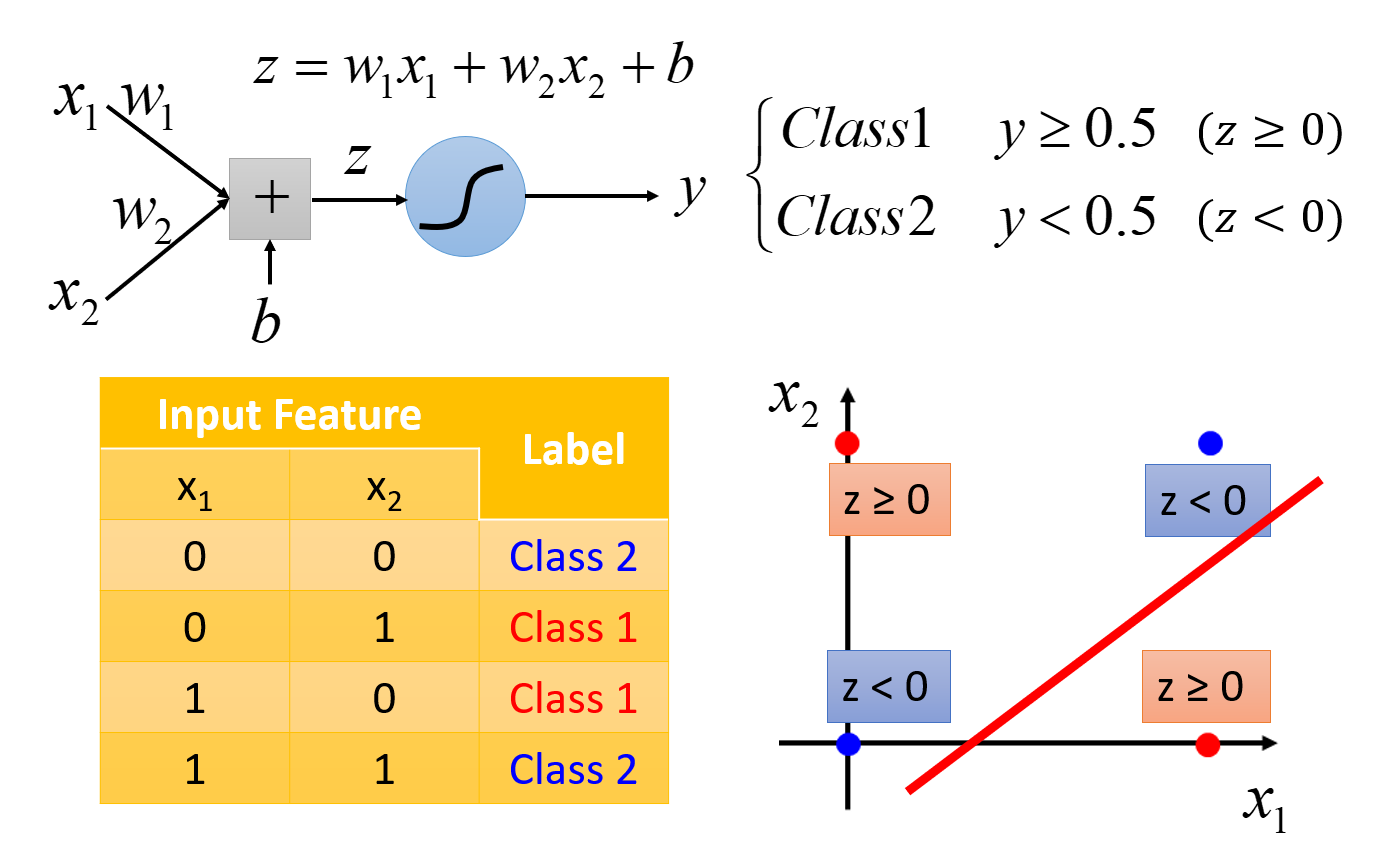
\includegraphics[scale=0.3]{pic/ClassTran.png}
  \label{fig:my_label}
\end{figure}

In this condition, we have to do \textbf{Feature Transformation}. It can solve this problem effectively. Again, this process is also expected to be done automatically by the machine. After doing Feature Transformation, we can use the transformed data to do Classification.

\begin{figure}[htbp]
  \centering
  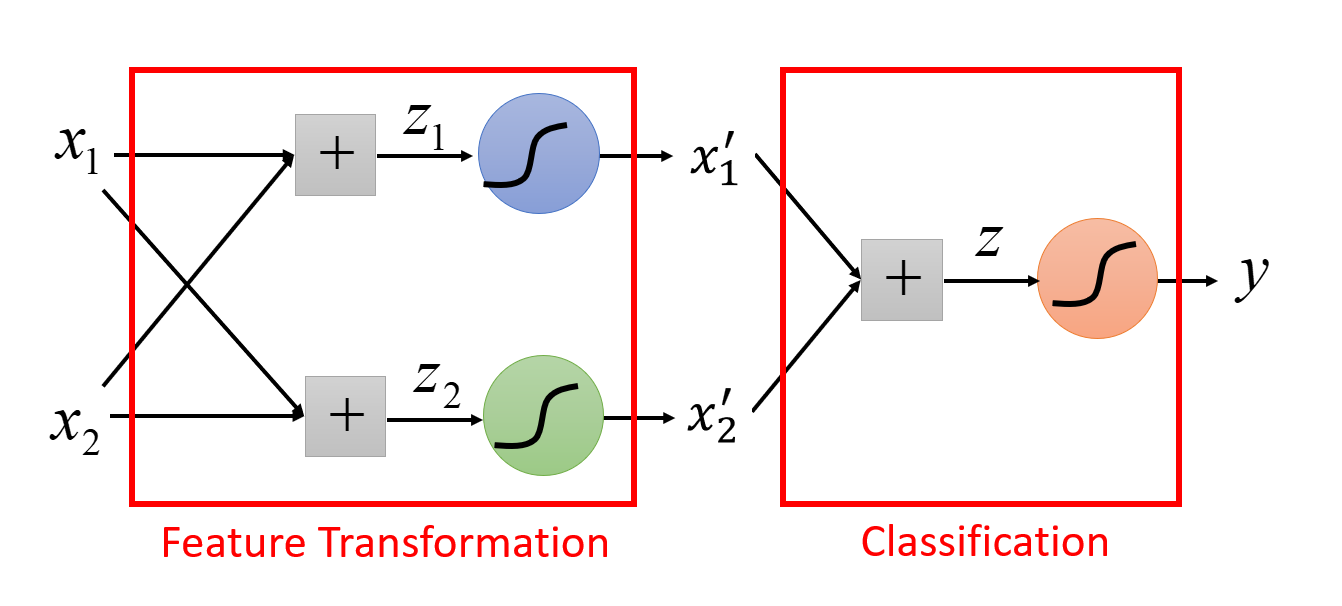
\includegraphics[scale=0.5]{pic/Feature Transformation .png}
  \label{fig:my_label}
\end{figure}

\section{Brief Introduction of Deep Learning}

Because this knowledge point has not important information. I quote other person's notes.

\begin{quoteblock}
    \href{https://blog.csdn.net/zn961018/article/details/116084191}{2020李宏毅机器学习笔记-Brief Introduction of Deep Learning}
\end{quoteblock}

\section{Backpropagation}

In practical applications, there are usually thousands of variables. To compute the gradients efficiently, we use \textit{\textbf{backpropagation}}.

In fact, the principle of backpropagation is Chain Rule. For example, there is a loss function we define:
$$
L(\theta) = \sum_{n=1}^N l^n(\theta)
$$
The partial derivative of this loss function is:
$$
\frac{\partial L(\theta)}{\partial w} = \sum_{n=1}^N\frac{\partial l^n(\theta)}{\partial w}
$$

We assume the neuron function is $z = w_1x^1+w_2x^2+b$. Then we can compute $\frac{\partial l}{\partial w}$.
$$
\frac{\partial l}{\partial w}=\frac{\partial z}{\partial w}\frac{\partial l}{\partial z}
$$
Obviously, $\frac{\partial z}{\partial w^1},\frac{\partial z}{\partial w^2}$ can easily be computed. But $\frac{\partial l}{\partial z}$ are not.

We generate $z$ and put it into another function like Sigmoid Function. Then $\frac{\partial l}{\partial z}$ can be represented in:
$$
\frac{\partial l}{\partial z} = \frac{\partial a}{\partial z}\frac{\partial l}{\partial a}
$$
In here $a = \sigma(z)$. Obviously, $\frac{\partial a}{\partial z} = a'$. We can assume that there have $n$ neuron nodes and denoted it with $v_1,\cdots,v_n$. It can be divided into:
$$
\frac{\partial l}{\partial a} = \sum_{i=1}^n\frac{\partial v_i}{\partial a}\frac{\partial l}{\partial v_i}
$$

After doing so many times, we finally approached to the output layer. The $\frac{\partial l}{\partial a_k}$ finally can be computed. Next we put all the answers back and get the $\frac{\partial l}{\partial w}$. We call it \textit{\textbf{Backpropagation}}.

\section{Tips for Training DNN}

If you get bad results on your model, there is a \textit{Recipe of Deep Learning}. Two questions:
\begin{itemize}
    \item Do you get Good Results on Training Data?
    \item Do you get Good Results on Testing Data?
\end{itemize}

\subsection{get Bad Results on Training Data}

In this subsection, there exist two ways to address this issue.

\subsubsection{New Activation Function}

We used Sigmoid Function before. But this function also have some side effection. For example, if we use big delta $\Delta w$. On the contrary, the gradient $\frac{\partial l}{\partial w}$ will be smaller. Because after a certain point the growth rate will become very small.

There are some other activation function:

\begin{tipsblock}{Rectified Linear Unit (ReLU)}
        $$
        \sigma(z) = \left\{\begin{matrix}z  & z>0\\0  & z\le 0\end{matrix}\right.
        $$
        The reason are: 1.The gradient can fast to compute. 2.Biological reason(paper given). 3.Infinite Sigmoid with different biases. 4.Vanishing gradient problem.
\end{tipsblock}

\begin{tipsblock}{ReLU - variant}
        Leaky ReLU:
        $$
        \sigma(z) = \left\{\begin{matrix}z  & z>0\\0.01z  & z\le 0\end{matrix}\right.
        $$
        \\
        Parametric ReLU:
        $$
        \sigma(z) = \left\{\begin{matrix}z  & z>0\\\alpha z  & z\le 0\end{matrix}\right.
        $$
\end{tipsblock}

\begin{tipsblock}{Maxout}
        From a neuron to another neuron it have so many weight named $w_i$. We put a certain number weights into a group named $G_i$.

        The activation is easily as:
        $$
        \alpha_{G_i} = \max(w_i) \quad w_i\in G_i
        $$

        By using Maxout like a map: $f:\mathbb R^n\to\mathbb R^m\quad(m = \text{size}(G))$

        After do it, the activation function just like linear $f(x) = x$ in $\max(w_i)$.
\end{tipsblock}

\subsubsection{Adaptive Learning Rate}

Like \textbf{RMSProp},\textbf{Momentum},\textbf{Adam}. It has already been mentioned above.

\subsection{Bad Results on Testing Data}

In this subsection, there exist three ways to address this issue.

\subsubsection{Early Stopping}

No more explanations.

\subsubsection{Regularization}

We will make a new loss function not only minimizing original cost but also close to zero in a set of weight. Make a function like this:
$$
L'(\theta) = L(\theta) + \lambda\frac{1}{2}\left \| \theta \right \|_{i} \quad(i = 1,2)
$$
$L(\theta)$ is original loss, $\theta$ is a set of weight $\{w_1,w_2,\cdots\}$. If $i=1$, we call it \textit{L1 regularization}. Other situations are same.

L2 regularization (also called Weight Decay):
$$
\left \| \theta \right \|_{2}=(w_1)^2+(w_2)^2+\cdots
$$
$$
\frac{\partial{L}^{\prime}}{\partial w}=\frac{\partial{L}}{\partial w}+\lambda w
$$
$$
w^{t+1}\to w^t - \eta \frac{\partial{L}^{\prime}}{\partial w} = (1-\eta\lambda)w^t-\eta\frac{\partial{L}^{\prime}}{\partial w}
$$

L1 regularization:
$$
\left \| \theta \right \|_{1}=|w_1|+|w_2|+\cdots
$$
$$
\frac{\partial{L}^{\prime}}{\partial w}=\frac{\partial{L}}{\partial w}+\lambda \text{sgn}(w)
$$
$$
w^{t+1}\to w^t - \eta \frac{\partial{L}^{\prime}}{\partial w} = w^t-\eta\frac{\partial{L}}{\partial w}-\eta\lambda\text{sgn}(w^t)
$$

\subsubsection{Dropout}

Each neuron has p\% to dropout before updating the parameters each time. we call it Dropout. For each mini-batch, we resample the dropout neurons.

If we try not dropout we also can make all the weights times (1-p)\%. It is can be proved in math. It can be used in activation function like quasi linear function.

\section{Why Deep}

In fact, each layer can be considered as a Modular calculation. That is why we use deep layer not one layer. It can give good result in less data rather than bad in one layer.

\begin{quoteblock}
    \href{https://blog.csdn.net/ygp12345/article/details/108902064}{why deep learning?我们为什么要使用深度学习?--ygpGoogle}
\end{quoteblock}

\section{Convolutional Neural Network}

CNN is widely working in image classify. And why CNN for image? There are some reasons in here.

If we use DNN to train the model, we will have a sea of weights like $1920\times 1080\times 3 \times l$. So big, isn't it? But from above section, each layer can be considered as a Modular calculation. We can split the image to many features. Such as bird's feather, beak. Every section only need a little size of pixels, and the same time, many neural input can share some same weight. Also, we can do subsampling to make the picture smaller.

CNN can be considered as -- do many times Convolution and Max Pooling then put Flatten(output) into DNN.

\subsection{Convolution}

Some patterns are much smaller than the whole image. How to address?

We use filter(info matrix) to get info in the filter size region like this picture:

\begin{figure}[htbp]
  \centering
  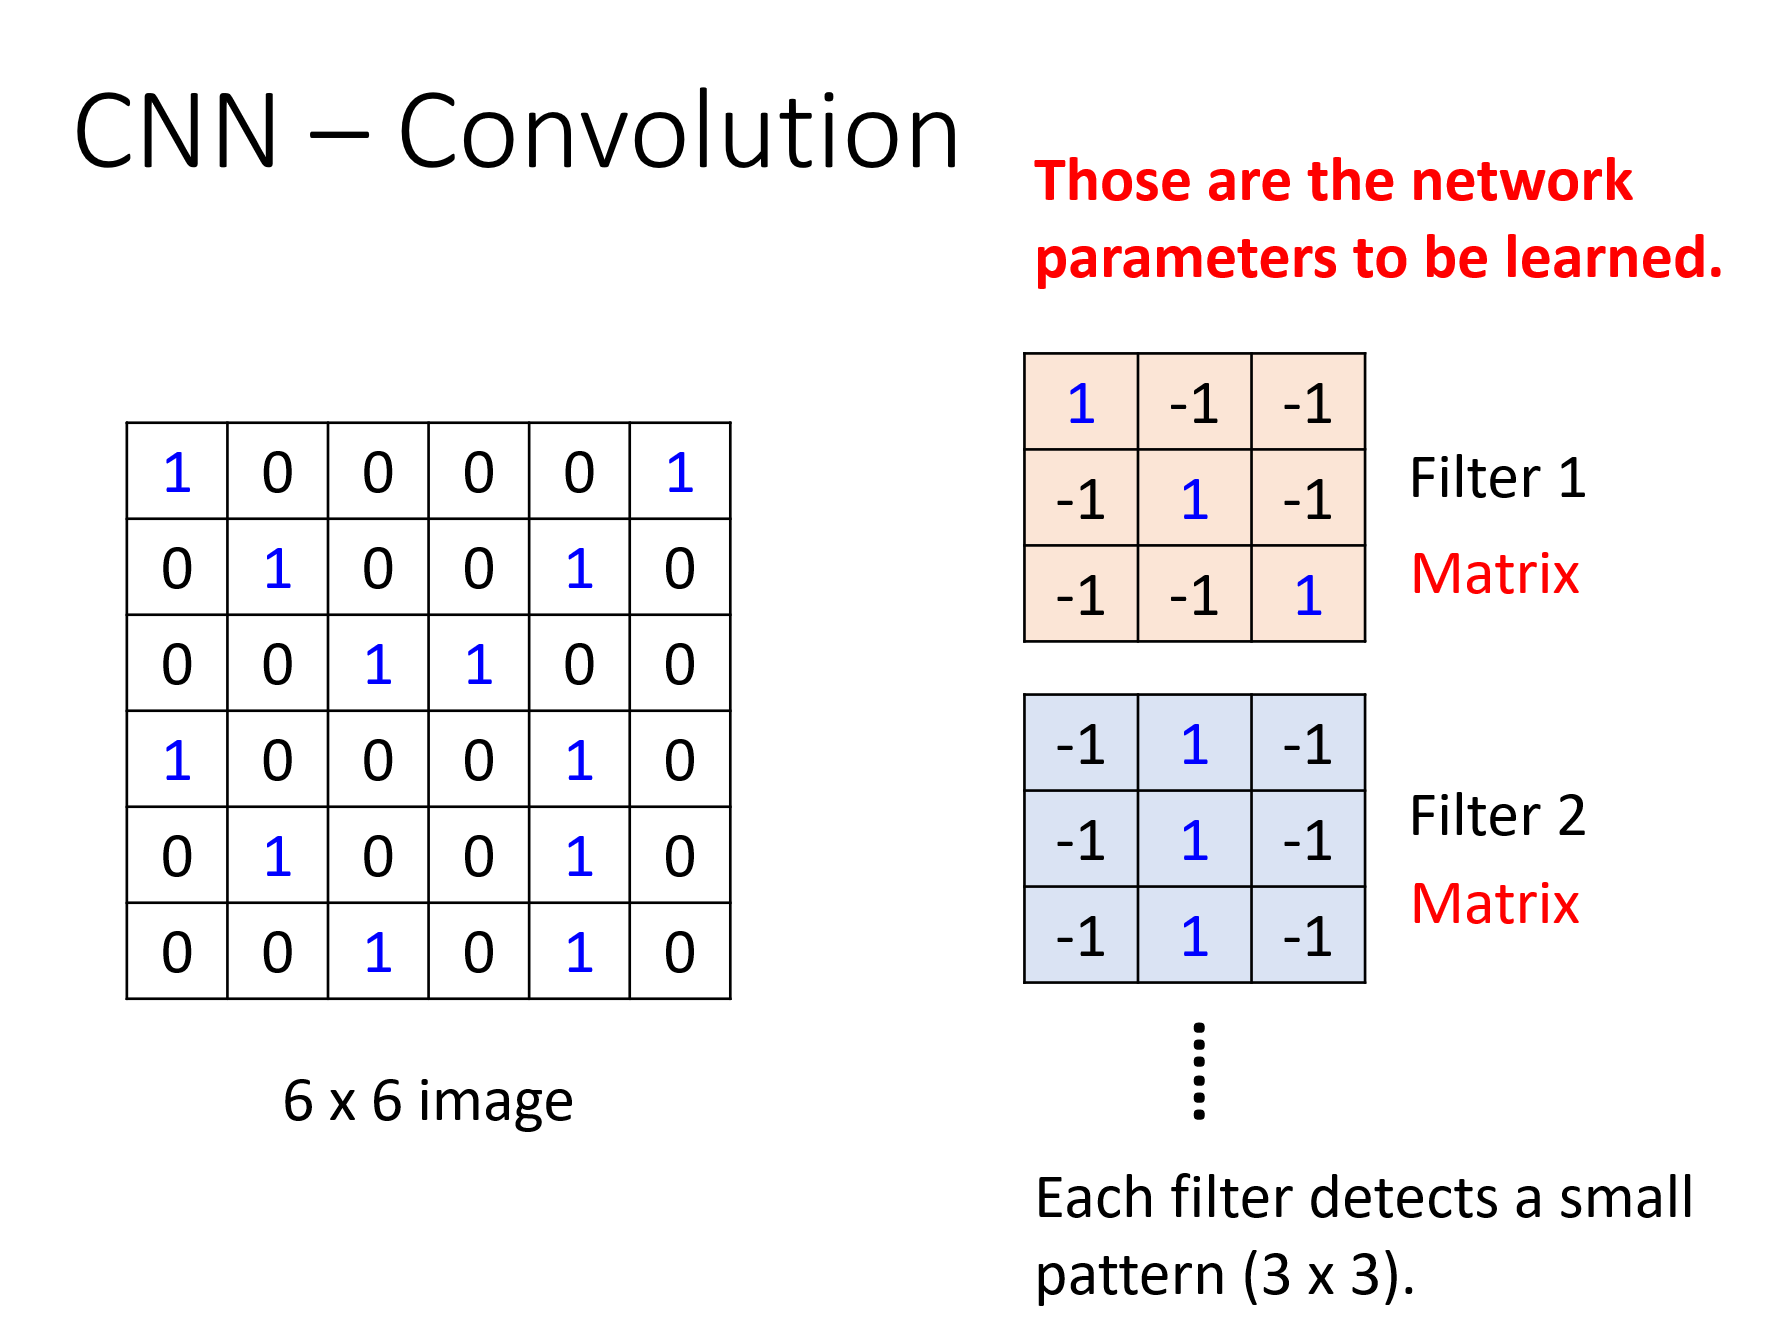
\includegraphics[scale=0.3]{pic/Property 1.png}
  \label{fig:my_label}
\end{figure}

The same patterns appear in different regions. Moving filter can work perfectly. Every area in size of filter can generate one info like this picture:

\begin{figure}[htbp]
  \centering
  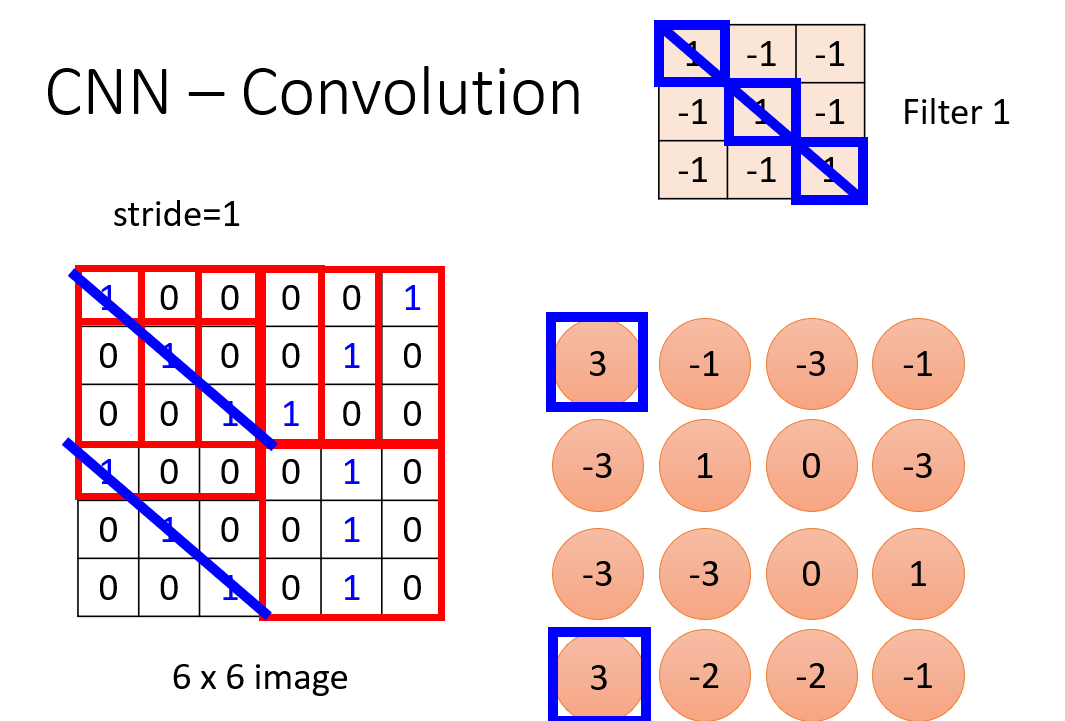
\includegraphics[scale=0.5]{pic/Property 2.png}
  \label{fig:my_label}
\end{figure}

Muti-filter are same. Such as Colorful image(every filter have three layers), we call the special muti-filter's vector 3-D tensor.

In this way, number of parameters can descent obviously. Have got tensor now, next issue is subsampling.

\subsection{Max Pooling}

Max Pooling is similar as Maxout. Assume we need half of size, put the tensor into many $2\times 2$ mini-tensor. Then get the maximum(also can use average or other) one as the feature mini-tensor.Therefore size of tensor turn into half.

In here we don't talk about that how the CNN can be trained. Toolkit can solve it. In other target, we maybe not apply Max Pooling like Alpha-Go in chess.

\section{Graph Neural Network}

In the modern time, graph is widely used in the deep learning. But how to put a graph into neural network as parameters. There are some issues in here:

\begin{itemize}
    \item How do we utilize the structures and relationship to help our model?
    \item What if the graph is larger, like $20$k nodes?
    \item What if we don‘t have the all the labels?
\end{itemize}

\subsection{Spatial-based GNN}

There are some terminologies and methods. 

\begin{colblock}[Definition of Aggregate]
    Make all neighbor's feature to update next layer's hidden state.
\end{colblock}

\begin{colblock}[Definition of Readout]
    Put all nodes' feature gathered to represent all of this graph.
\end{colblock}

\begin{markerblock}
    List only a small number of easy-to-understand methods.
\end{markerblock}

\subsubsection{Neural Networks for Graph (NN4G)}

We denoted every node as $v_i$. Assume that $v_1$ only connect with $v_2,v_3,v_4$. And every node have there own parameter denoted $x_i$, it's weight denoted as $w_i$. $h_i^j$ is on i-th node j-th layer's value.

$$
h^0_1 = w_1 x_1
$$

$$
h^i_1 = \hat{w}_{1,i-1}(h^{i-1}_{2}+h^{i-1}_{3}+h^{i-1}_{4})\quad (i>1)
$$

We define $X_i = \frac{\sum_{k=1}^n h^i_k}{n}$. And Readout of it is:
$$
z = \sum^n w_iX_i
$$
It need to train out.

I want to be lazy. So I only put other into list.
\begin{itemize}
    \item Diffusion-Convolution Neural Network (DCNN)
    \item Diffusion Graph Convolution (DGC)
    \item Mixture Model Networks (MoNET)
    \item GraphSAGE
    \item \textbf{Graph Attention Networks (GAN)}
    \item Graph Isomorphism Network (GIN)
\end{itemize}

Because of my poor knowledge, I have to give up this section...

\section{Recurrent Neural Network}

RNN is like a DNN with memory. The data in the RNN cell can be remembered and used in next RNN cell. There are some methods of RNN:

\begin{itemize}
    \item SimpleRNN
    \item Bidirectional RNN
    \item Long Short-term Memory (LSTM)
\end{itemize}


As its name SimpleRNN, the structure of SimpleRNN is simple. It like DNN only put in some memory unit in it. This is SimpleRNN figure:

\newpage

\begin{figure}[htbp]
  \centering
  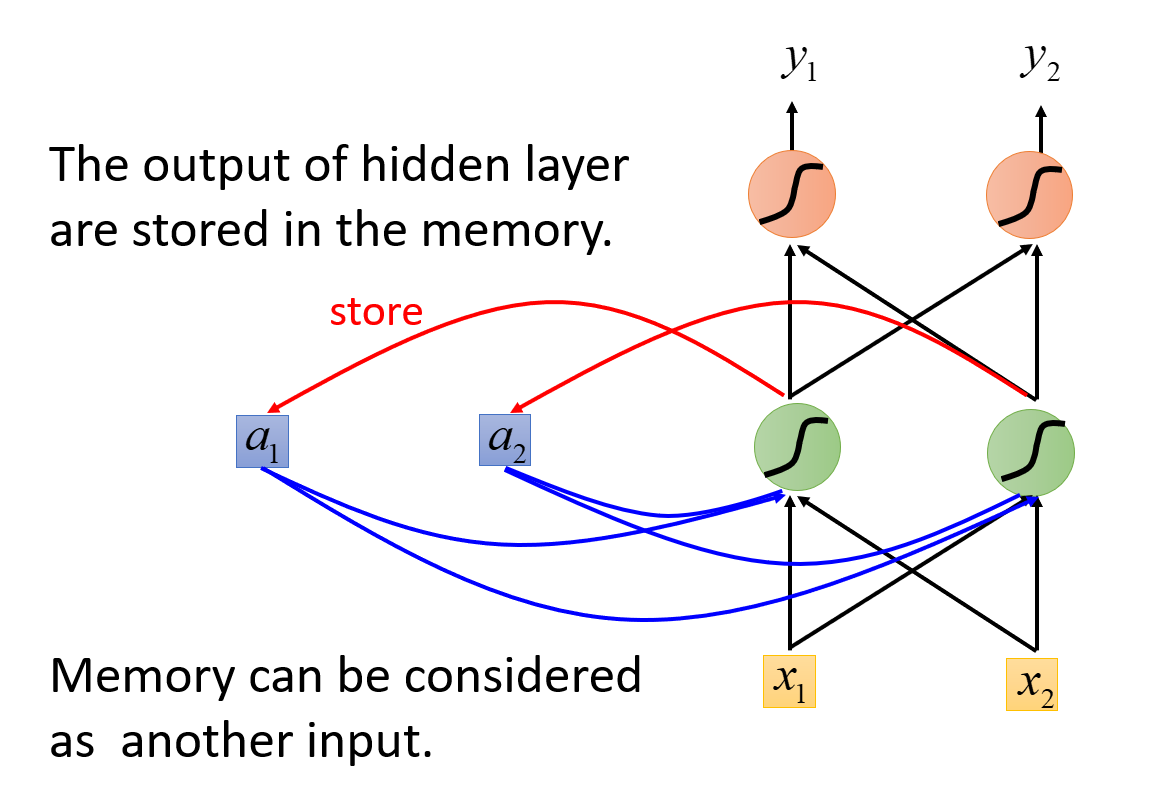
\includegraphics[scale=0.5]{pic/srnn.png}
  \label{fig:my_label}
\end{figure}

Every data process through mid activation function will put in the memory unit and will use in next RNN as input's weight times on the input. Of course it can be deep.

Bidirectional RNN is like entering input in positive and negative order and averaging the values in their memory cells.

Long Short-term Memory is what we need to know. In fact, LSTM have three gates:Input gate,Forget gate and Output gate. We use Sigmoid Function as activation function to control it open or not. The structure like this:

\begin{figure}[htbp]
  \centering
  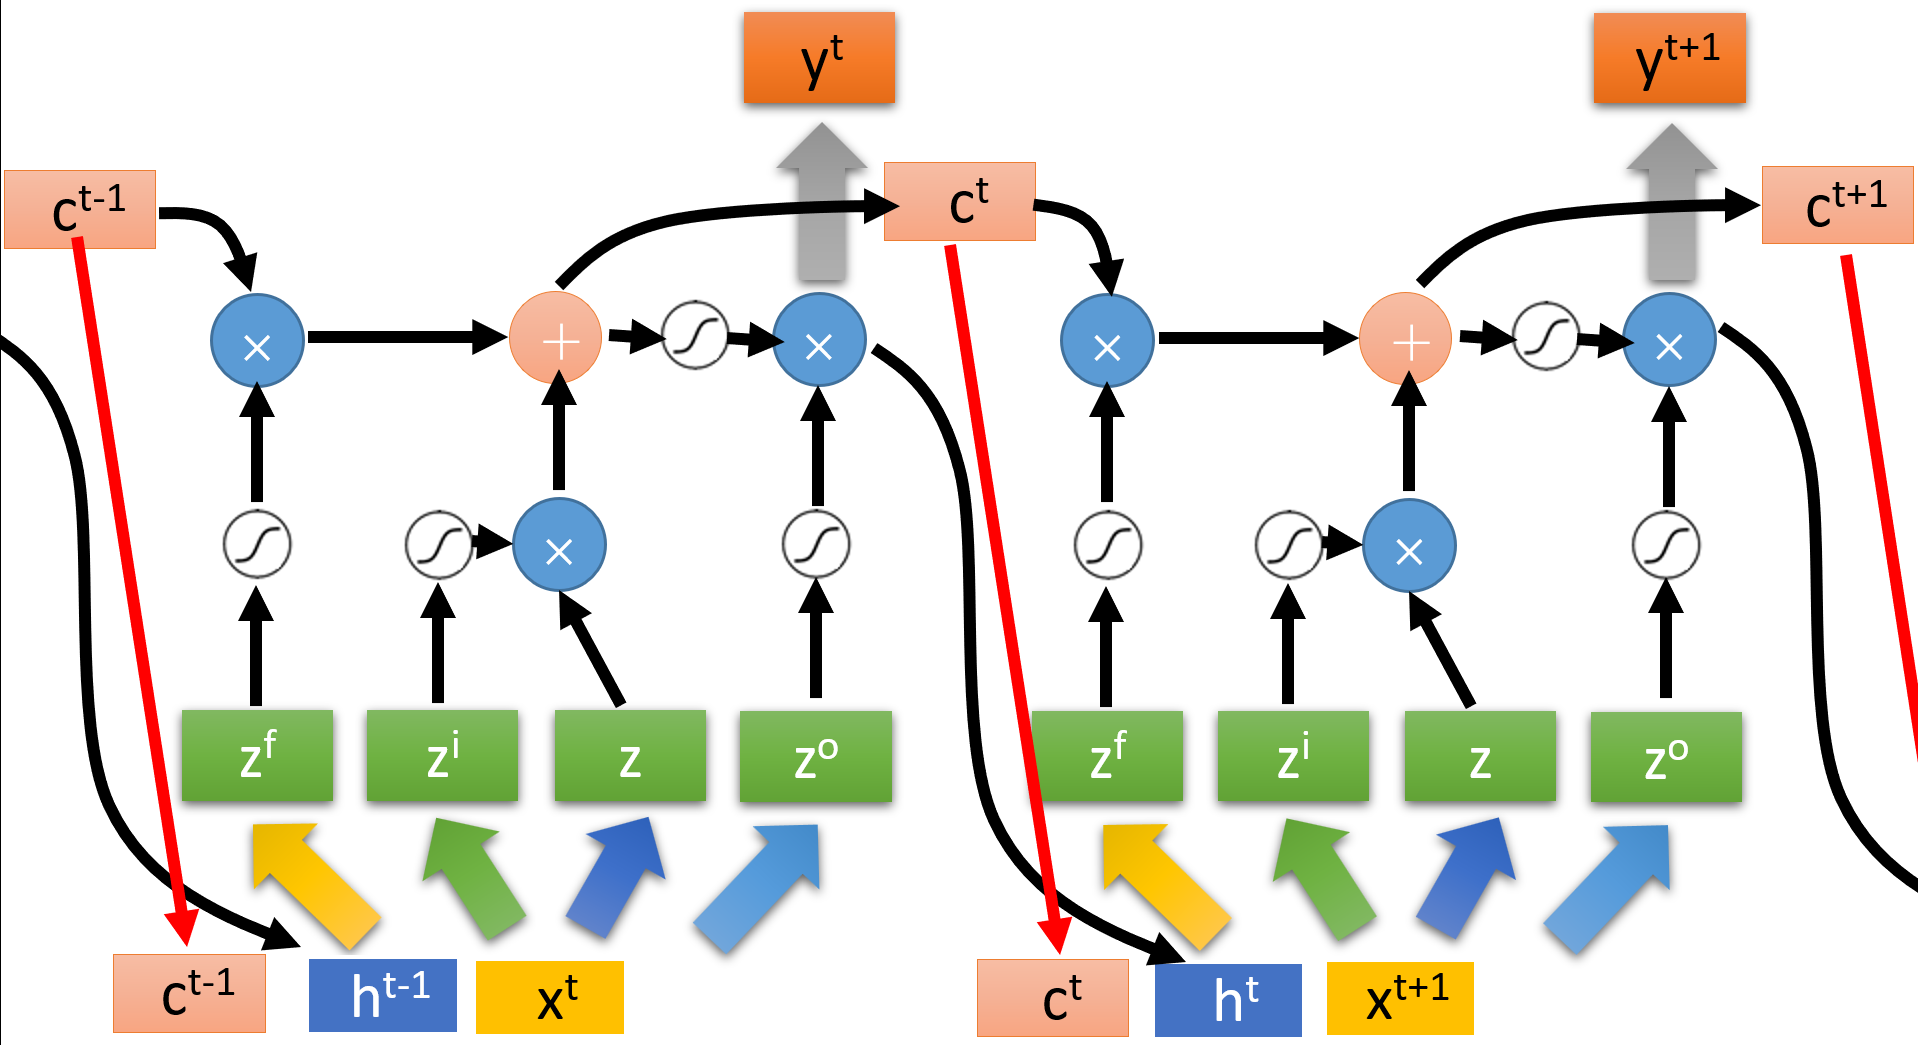
\includegraphics[scale=0.5]{pic/lstm.png}
  \label{fig:my_label}
\end{figure}

But RNN have a big issue:The error surface is rough. The error surface is either very flat or very steep. But LSTM maybe can address this issue.

\section{Semi-supervised Learning}

\begin{colblock}[Definition of Semi-supervised Learning]
    There is a set of unlabeled data, usually far more than labeled data. Using unlabeled data to develop model which trained by labeled. It is called Semi-supervised Learning.
\end{colblock}

Why semi-supervised learning helps? The \textbf{distribution} of the unlabeled data tell us something.

\subsection{Semi-supervised Learning for Generative Model}

For example, Given labeled training examples $x^r \in C_1,C_2$. Looking for most likely prior probability $P(C_i)$ and class-dependent probability $P(x|C_i)$. $P(x|C_i)$ is a Gaussian parameterized by $\mu^i$ and $\sigma$. Then we have a label trained model. But the model must not exactly. Therefore we use unlabeled data $x^u$ to help re-estimate its parameters.

The algorithm converges eventually, but the initialization influences the results.
 
\begin{propblock}[How To Do Semi-supervised Generative]
    Initialization: $\theta = \{P(C_1),P(C_2),\mu^1,\mu^2,\Sigma\}$
    
    Step 1: Compute the posterior probability of unlabeled data $P_\theta(C_1|x^u)$ (Depending on model $\theta$).

    Step 2: Update model. $N$: total number of examples. $N_1$: number of examples belonging to $C_1$.
    $$
    P(C_1) = \frac{N_1+\sum_{x^u}P(C_1|x^u)}{N}
    $$
    And so on. Finally update whole $\theta$ then back to step 1. The new loss function is:
    $$
    \log L(\theta) = \sum_{(x^r,\hat y^r)}\log P_\theta(x^r|\hat y^r) + \sum_{x^u} \log P_\theta(x^u)
    $$
    $$
    P_\theta(x^u) = P_\theta(x^u|C_1)P(C_1) + P_\theta(x^u|C_2)P(C_2)
    $$
\end{propblock}

\subsection{Semi-supervised Learning Low-density Separation}

The low-density separation hypothesis assumes that the data is either black or white, and there is a significant gap between the two categories of data, that is, at the boundary between the two categories of data density is very low (that is, the volume of data is very good).

The method of self-training is very intuitive. First, it trains a model based on the data with labels. It inputs the data without labels as test data, and gets the data without labels as labels, then a part of the data with a false label is transferred to the data with a label, in the training, cycle back and forth.

\begin{markerblock}
    This method could not use in regression. And the false label must using hard tag like $[1,0]$ not $[0.79,0.21]$.
\end{markerblock}

\subsubsection{Entropy-based Regularization}

A regularization method make label have a big difference. The entropy can be get by:

$$
E(y^u) = - \sum_{m=1}^n y^u_m \ln (y^u_m)
$$

So we can use regularization to make the loss function better:

$$
L = \sum_{x^r} C(y^r,\hat y^r) + \lambda \sum_{x^u} E(y^u)
$$

\subsection{Semi-supervised Learning Smoothness Assumption}

Smoothness assumption: if the input $x$ is similar, then the label values $\hat y$ Should also be similar. But this assumption is not accurate enough, so there are the following strict assumptions:

\begin{itemize}
    \item x is not uniform. 
    \item If $x^1$ and $x^2$ are close in a high density region, $y^1$ and $y^2$ are the same.
\end{itemize}

\subsubsection{Cluster and then Label}

An intuitive approach is to cluster the data first to see where the unlabeled data falls, and then to mark it. However, if the image is manipulated, it is not possible to cluster the image by pixels alone, and such a clustering method is often not good. In this case, we can use deep autoencoder to extract the features of the image, the better result can be obtained by clustering images with features

\subsubsection{Graph-based Approach}

All the data points are made into a graph, if the two points on the graph can be connected, then the label between them is the same. So how do you form a graph, well, some graphs are natural, like links between web pages, or citations between papers, but sometimes you have to build them yourself.

\section{Unsupervised Learning - Word Embeddin}

This is a concrete example of unsupervised learning, so I won't take notes. Here is a quote from someone else's notes.

\begin{quoteblock}
    \href{https://zhuanlan.zhihu.com/p/396517227}{李宏毅机器学习课程笔记-15.4无监督学习之Word Embedding}
\end{quoteblock}

\section{Explainable ML}

Why we need Explainable ML? Neural network usually like a black box. To get the reason why machine can get this answer, we need to make it explainable.

There are two types of explainable. One is local explainable, which generally refers to how the machine interprets the example (for example, in the classification problem, how the machine divides a picture of a cat into cats) The other is global explainable, which generally refers to how the machine judges a population's characteristics (for example, in classification problems, what the machine thinks a cat looks like).

\subsection{Local Explanation}

Split the model input object into components, remove or adjust the value of a component, which is important if the change in the component can lead to significant decision changes in the model.


\begin{propblock}[Detection Based on Sliding Window]
    Sliding a gray square on the input image to block the local area, and observing which position is blocked by the gray square can lead to model error judgment.
\end{propblock}

\begin{propblock}[Detection Based on Gradient]
    $$
    (x_1,\cdots,x_i,\cdots,x_n)\to(x_1,\cdots,x_i+\Delta x,\cdots,x_n)
    $$
    $$
    y_k \to y_k + \Delta y
    $$

    For each dimension, we do a little effect $\Delta x$. The prediction $y_k$ will be $y_k + \Delta y$. Then compute the gradient that we can get the more important part.
\end{propblock}

But this method have two issues:

\begin{itemize}
    \item There is a gradient saturation.
    
    For example, the length of an elephant's trunk may be a key factor in determining whether an image is an elephant. If the length of the trunk in an image exceeds a threshold, it is considered an elephant, then the partial derivative of the output to the length of the nose is very small.

    \item May be attacked maliciously

    Some artificial noise can destroy the direction of attention of the machine.
\end{itemize}

\subsection{Global Explanation}

Let the model tell us what the input should look like for the highest possible probability value for a certain category.
$$
x^* = arg \max_{x} y_i
$$

\subsection{Activation Maximization}

Use some regular method like L1,L2 regulation.

$$
x^* = arg \max_x y_i + R(x)
$$

\subsection{Using Generator}

Using some generation algorithms, such as VAE, GAN... train a good image generator. Because for the generator, can enter a random vector $z$ to generate a picture $x = G(z)$, and then use the idea of method 1. Then the question becomes:
$$
x^* = arg \max_x y_i \to z^* = arg \max_z y_i
$$
The whole idea is to replace the constraints $R(x)$ of Method 1 with a generator.


\subsection{Using Explainable Model to Explanation}

Some easy-to-explain models (such as Linear Model, Decision Tree, etc.) are used to simulate complex models (such as neural networks) for interpretation. However, the simple model is often limited in representation ability, and can not fully simulate the highly nonlinear model, only to simulate the local characteristics of the complex model. So this approach is really a Local Explanation.

\begin{itemize}
    \item Local Interpretable Model agnostic-Explanation (LIME)
    \item Decision tree regularization
\end{itemize}

\section{Attack ML Models}

The classifiers that are robust to noises and work “most of the time” is not sufficient. We want the classifiers that are robust the inputs that are built to fool the classifier.

We define some symbol: $y^0$: is original picture through network's answer. $y'$: is original picture plus noise's answer. $x^0$: is original picture's vector. $x'$: is original picture plus noise's vector.

Training: 
$$
L_{train}(\theta) = C(y^0,y^{true}) \quad (x\quad\text{fixed})
$$

Non-targeted Attack:
$$
L'(x) = - C(y',y^{true}) \quad (\theta\quad\text{fixed})
$$

Targeted Attack: 
$$
L(x') = -C(y',y^{true}) + C(y',y^{false})
$$

Constraint:
$$
d(x^0,x') \le \varepsilon
$$
$$
d_2 := \left\| x^0 - x'\right\|_2 = \sum^n (\Delta x_i)^2
$$
$$
d_{inf} := \left\| x^0 - x'\right\|_{inf} = \max_{i\in n}(\Delta x_i)
$$

\begin{propblock}[How to Train it]
    Just like training a neural network, but network parameter $\theta$ is replaced with input $x'$.
    $$
    x^* = arg \min L(x')
    $$
    If $d(x^0,x^t) > \varepsilon$, do $x^t\gets fix(x^t)$. $fix(x) :=$ For all $x$ fulfill $d(x^0,x) \le \varepsilon$ return the one closest to $x^t$.
\end{propblock}

There are other attack approaches:
\begin{itemize}
    \item FGSM
    \item Basic iterative method
    \item L-BFGS
    \item Deepfool
    \item JSMA
    \item C\&W 
    \item …… only list a few
\end{itemize}

Adversarial Attack cannot be defended by weight regularization, dropout and model ensemble. There are two types of defense:

\begin{itemize}
    \item \textbf{Passive defense}: Finding the attached image without modifying the model 
    \item \textbf{Proactive defense}: Training a model that is robust to adversarial attack
\end{itemize}

\section{Network Compression}

How to apply the ability of AI to these mobile devices and embedded devices is an urgent problem to be solved. The traditional deep network model is too big and has too many parameters to be used directly. Is it possible to simplify the structure and parameters of the network so that the model can run on mobile phones and microprocessors?

\subsection{Network Pruning}

Some weights or neural in the network are useless. Pruning is a method to address this issue. Cut some useless weight/neural out, make model petite. 

Usually, putting neural out is famous way. Because reducing weight will make the network structure become irregular, difficult to achieve from the code level, it is difficult to parallelize. With neuron reduced, the network is still normalized.

\subsection{Knowledge Distillation}

His idea was to replicate the performance of a large network over a small network, the so-called teacher-student model. Note that the monitor signal for the student network is the output of the teacher network, not the actual label.

\subsection{Parameter Quantization and Architecture Design}

\begin{quoteblock}
    \href{https://zhuanlan.zhihu.com/p/122977022}{2020机器学习前沿技术----network compression--stephon}
\end{quoteblock}

\section{Conditional Generation by RNN and Attention}

\begin{quoteblock}
    \href{https://zhuanlan.zhihu.com/p/388521961}{李宏毅 conditional generation by RNN \& attention 笔记
--小范同学}
\end{quoteblock}












\end{document}
艾萨克·牛顿(1643年1月4日$\sim$1727年3月31日),爵士,英国皇家学会会长,英国著名的物理学家、数学家,百科全书式的“全才”,著有《自然哲学的数学原理》《光学》。他在1687年发表的论文《自然定律》里,对万有引力和三大运动定律进行了描述。这些描述奠定了此后三个世纪里物理世界的科学观点,并成为了现代工程学的基础。他通过论证开普勒行星运动定律与他的引力理论间的一致性,展示了地面物体与天体的运动都遵循着相同的自然定律;为太阳中心说提供了强有力的理论支持,并推动了科学革命。牛顿曾经说过一句很著名的话

\begin{quoteblock}
    如果说我看得远,那是因为我站在巨人的肩上。

    \rightline{——牛顿}
\end{quoteblock}

牛顿第一定律的内容为

\begin{thmblock}[牛顿第一定律]
    任何一个物体总是保持静止状态或者匀速直线运动状态,直到有作用在它上面的外力迫使它改变这种状态为止。
\end{thmblock}

我们在初中和高中都已经学过了牛顿第一定律,因此不在此做过多阐释。但值得指出的是
\begin{tipsblock}{补充}
    \begin{itemize}
        \item 牛顿第一定律给出了一个没有加速度的参考系——惯性系,使人们对物理问题的研究和物理量的测量有意义,从而使它成为整个力学甚至物理学的出发点。牛顿第二、第三定律以及由牛顿运动定律建立起来的质点力学体系,如动量定理、动量守恒定律、动能定理等,只对惯性系成立。
        \item 牛顿第一定律是其他原理的前提和基础。第一定律中包含的基本概念,奠定了经典力学的概念基础,从而使它处于理论系统中第一个原理的前提地位,这表现在:
              \begin{enumerate}
                  \item 首次批驳了延续两千多年的亚里士多德等人错误的力的概念,为确立正确的力的概念奠定了基础。
                  \item 第一次科学地给出了力的定性定义(含力的本质和力的效果)。
                  \item 第一次提出了经典力学的几个基本概念,为第二、第三定律以及由牛顿运动定律建立起来的质点力学体系原理奠定了概念基础。
              \end{enumerate}
    \end{itemize}
\end{tipsblock}

使用牛顿第一定律时需要注意如下情况:

\begin{markerblock}
    牛顿第一定律只适用于惯性参考系。在质点不受外力作用时,能够判断出质点静止或作匀速直线运动的参考系一定是惯性参考系,因此只有在惯性参考系中牛顿第一运动定律才适用。
    牛顿第一定律在非惯性参考系(即有加速度的系统)中不适用,因为不受外力的物体,在该参考系中也可能具有加速度,这与牛顿第一定律相悖。
\end{markerblock}

接下来我们学习牛顿第二定律。牛顿指出,力是改变物体运动状态的原因;牛顿第二定律用数学公式刻画了力和物体运动状态改变的关系。
\begin{thmblock}[牛顿第二定律]
    动量为$\vec{p}$的质点,在外力的作用下,其动量随时间的变化率同该质点所受的外力成正比,并与外力的方向相同。用公式表达为
    $$
        \vec{F}=\frac{\text{d} \vec{p}}{\text{d} t}
    $$
\end{thmblock}

这是牛顿在《自然哲学的数学原理》发表的原始表述。为了理解这一式子,我们给出动量的定义:
\begin{defblock}[动量的定义]
    动量$p$是与物体的质量$m$和速度$v$相关的物理量。动量为矢量,由下式给定
    $$
        \vec{p}=m\times \vec{v}
    $$
\end{defblock}

牛顿第二定律的推论,也即其常见表述为
\begin{colblock}[牛顿第二定律的常见表述]
    物体加速度的大小与合外力成正比,与物体质量成反比(与物体质量的倒数成正比)。加速度的方向与合外力的方向相同。用公式表示即为
    $$
        \vec{F}=m\times \vec{a}
    $$
\end{colblock}

现在我们快速地证明牛顿第二定律的两种表述是等价的。
\begin{proof}
    牛顿第二定律指出,
    \begin{equation}
        \vec{F}=\frac{\text{d} \vec{p}}{\text{d} t}\label{def:f}
    \end{equation}
    再根据动量的定义,
    \begin{equation}
        \vec{p}=m\times \vec{v}
    \end{equation}
    因此有,
    \begin{equation}
        \frac{\text d \vec{p}}{\text d t}=\frac{\text d \vec{m\times\vec{v}}}{\text d t}=m\times \vec{a}\label{derivative}
    \end{equation}
    从等式(\ref{def:f})和等式(\ref{derivative})可以得出,
    $$
        \vec{F}=m\times \vec{a}
    $$
\end{proof}

了解牛顿第二定律后,思考如下命题的正确性。
\begin{propblock}[命题]
    做匀速圆周运动的物体必定受力。
\end{propblock}

接下来做一道简单的关于牛顿第二定律的题。

\begin{quesblock}
    已知一个物块的质量为$10kg$,若物块以$10m/s$的速度冲上滑板,滑板的动摩擦因数$\mu=0.1$,请问物块需要多久会静止?(重力加速度$g$的大小为$g=10m/s^2$)
\end{quesblock}

\begin{solblock}
    \begin{solution}
        \begin{equation*}
            \begin{aligned}
                F=\mu m g            \\
                a =\frac{F}{m}=\mu g \\
                t = \frac{v}{a}=10s
            \end{aligned}
        \end{equation*}
    \end{solution}
\end{solblock}
